\documentclass[twocolumn,preprintnumbers,amsmath,amssymb,superscriptaddress]{revtex4}
%\usepackage[pdftex]{graphicx}

\usepackage{amsmath,amsfonts,amssymb}
\usepackage[english]{babel} 
\usepackage[latin1]{inputenc} 
\usepackage[T1]{fontenc}
\usepackage{color}
\usepackage{float}
\usepackage{verbatim}
\usepackage{graphicx}
\usepackage{bm}
\usepackage{mathtools}
\usepackage{stmaryrd} 
\usepackage{anyfontsize}


%\usepackage{epstopdf}
%\usepackage{array}
%\usepackage{tabularx}
%\usepackage{multirow}
\usepackage{color}
%\usepackage{multibox}
%\usepackage{rotating}
%\usepackage{lineno}
%\usepackage[left]{lineno}
%\usepackage[comma,sort&compress]{natbib}
%\usepackage{authblk}
%\usepackage{multicol}

%\bibliographystyle{ieeetr}


%\linenumbers
%\setlength\linenumbersep{3pt}

\begin{document}


\author{Justin D. Yeakel} \affiliation{School of Natural Sciences, University
  of California, Merced, Merced, CA 95340, USA}

\author{Christopher P. Kempes} \affiliation{The Santa Fe Institute, 1399 Hyde
  Park Road, Santa Fe, NM 87501, USA}

\author{Sidney Redner} \affiliation{The Santa Fe Institute, 1399 Hyde Park
  Road, Santa Fe, NM 87501, USA}

\title{The dynamics of starvation and recovery}%: Eco-evolutionary feedbacks}

%\author{Justin D. Yeakel${}^{1,2,*}$, Christopher P. Kempes${}^{2}$, \& Sidney Redner${}^{2,3}$ \\ \\
%${}^1$School of Natural Science, University of California Merced, Merced, CA \\
%${}^2$The Santa Fe Institute, Santa Fe, NM \\
%${}^3$Department of Physics, Boston University, Boston MA \\
%${}^*$To whom correspondence should be addressed: jdyeakel@gmail.com
%}


\begin{abstract}

The eco-evolutionary dynamics of species is fundamentally linked to the
energetic constraints of its constituent individuals.  Of particular
importance are the tradeoffs between reproduction and the dynamics of
starvation and recovery in resource-limited environments.  To elucidate the
consequences of this tradeoff, we introduce a minimal nutritional
state-structured model that incorporates two classes of consumer:
nutritionally replete consumers that reproduce, and undernourished,
non-reproducing consumers that are susceptible to mortality.  As a function
of the transition rates between these replete and undernourished states that
are determined by the presence or absence of resources, the consumer
populations can either undergo cyclic dynamics or reach a steady state.  We
obtain strong constraints on starvation and recovery rates by deriving
allometric scaling relationships and find that population dynamics subject to
these constraints can approach the cyclic regime but are typically driven to
a steady state.  Moreover, we find that these rates fall within a `refuge' in
parameter space, where the probability of extinction of the consumer
population is minimized.  Thus we identify a potential mechanism that may
both drive and constrain the dynamics of animal populations.  Our model
provides a natural framework that predicts maximum body size for mammals by
determining the relative stability of an otherwise homogeneous population to
a mutant population with altered percent body fat.  For body masses
$\lesssim 10^7$g, individuals with increased energetic reserves can invade
resident populations, and vice versa for body mass $\gtrsim 10^7$g, thus
providing a principled mechanism for a within-lineage driver of Cope's rule.

\end{abstract}

%\newpage

%\begin{multicols}{2}

\maketitle

\section*{Introduction}
The behavioral ecology of all organisms is influenced by the energetic state
of individuals, which directly influences how they invest reserves in
uncertain environments.  Such behaviors are generally manifested as tradeoffs
between investing in somatic maintenance and growth, or allocating energy
towards reproduction~\cite{Martin:1987dl,Kirk:1997cc,Kempes:2012hy}.  The
timing of these behaviors responds to selective pressure, as the choice of
the investment impacts future
fitness~\cite{Mangel:1988uaa,Mangel:2014kz,Yeakel:2013hi}.  The influence of
resource limitation on an organism's ability to maintain its nutritional
stores may lead to repeated delays or shifts in reproduction over the course
of an organism's life.

The balance between (a) somatic growth and maintenance, and (b) reproduction
depends on resource availability~\cite{Morris:1987eo}.  For example, reindeer
invest less in calves born after harsh winters (when the mother's energetic
state is depleted) than in calves born after moderate
winters~\cite{Tveraa:2003fq}.  Many bird species invest differently in broods
during periods of resource scarcity compared to normal
periods~\cite{Daan:1988va,Jacot:2009dv}, sometimes delaying or even foregoing
reproduction for a breeding
season~\cite{Martin:1987dl,Stearns:1989ip,Barboza:2002in}.  Even freshwater
and marine zooplankton have been observed to avoid reproduction under
nutritional stress~\cite{Threlkeld:1976ih}, and those that do reproduce have
lower survival rates~\cite{Kirk:1997cc}.  Organisms may also separate
maintenance and growth from reproduction over space and time: many salmonids,
birds, and some mammals return to migratory breeding grounds to reproduce
after one or multiple seasons in resource-rich environments where they
accumulate nutritional
reserves~\cite{Weber:1998jg,Mduma:1999cp,Moore:2014hi}.

Physiology also plays an important role in regulating reproductive
expenditures during periods of resource limitation.  The data collected thus
far has shown that diverse mammals (47 species in 10 families) exhibit
delayed implantation, whereby females postpone fetal development (blastocyst
implantation) until nutritional reserves can be
accumulated~\cite{Mead:1989dt,Sandell:1990kw}.  Many other many species
(including humans) suffer irregular menstrual cycling and higher abortion
rates during periods of nutritional stress~\cite{Bulik:1999eo,Trites:2003cc}.
In the extreme case of unicellular organisms, nutrition is unavoidably linked
to reproduction because the nutritional state of the cell regulates all
aspects of the cell cycle \cite{Glazier:2009hq}.  The existence of so many
independently evolved mechanisms across such a diverse suite of organisms
highlights the importance and universality of the fundamental tradeoff
between somatic and reproductive investment.  However the general dynamic
implications of these constraints are unknown.

Though straightforward conceptually, incorporating the energetic dynamics of
individuals~\cite{Kooi2000} into a population-level
framework~\cite{Kooi2000,Sousa:2010ez} presents numerous mathematical
obstacles~\cite{Diekmann:2010da}.  An alternative approach involves modeling
the macroscale relations that guide somatic versus reproductive investment in
a consumer-resource system.  For example, macroscale Lotka-Volterra models
assume that the growth rate of the consumer population depends on resource
density, thus \emph{implicitly} incorporating the requirement of resource
availability for reproduction~\cite{murdoch:2003}.

In this work, we adopt an alternative approach in which we \emph{explicitly}
account for resource limitation and the subsequent effects of starvation.
Namely, only individuals with sufficient energetic reserves can reproduce.
Such a constraint leads to reproductive time lags due to some members of the
population going hungry and then recovering.  Additionally, we incorporate
the idea that reproduction is strongly constrained allometrically
\cite{Kempes:2012hy}, and is not generally linearly related to resource
density.  As we shall show, these constraints influence the ensuing
population dynamics in dramatic ways.


\section*{Nutritional state-structured model (NSM)}
We begin by defining a minimal Nutritional State-structured population Model (NSM), where the consumer population is partitioned into two states: (a) an energetically replete (full) state $F$, where the consumer reproduces at a constant rate $\lambda$ and does not die from starvation, and (b) an energetically deficient (hungry) state $H$, where the consumer does not reproduce but dies by starvation at rate $\mu$.  
The underlying resource $R$ evolves by logistic growth with an intrinsic growth rate $\alpha$ and a carrying capacity equal to one.  
Consumers transition from the full state $F$ to the hungry state $H$ at a rate $\sigma$---the starvation rate---and also in proportion to the absence of resources $(1-R)$.  Conversely, consumers recover from state $H$ to state $F$ at rate $\rho$ and in proportion to $R$. 
Resources are also eaten by the consumers---at rate $\rho$ by hungry consumers and at rate $\beta<\rho$ by full consumers.  
This inequality accounts for hungry consumers requiring more resources to replace lost body tissue.  
The NSM represents a fundamental extension of the idealized starving random walk model of foraging, which focuses on resource depletion, to include reproduction and resource replenishment~\cite{Benichou:2014wu,Benichou:2016wl,Chupeau:2016jf}.


\begin{figure*}[ht]
\centering
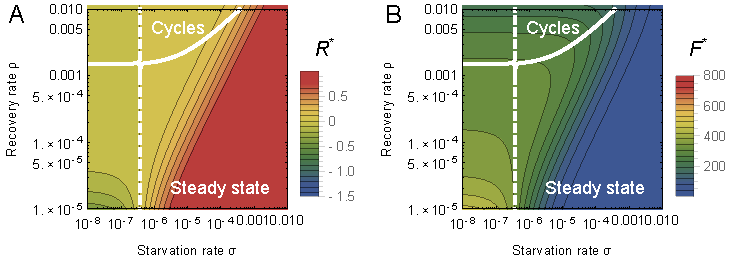
\includegraphics[width=0.75\textwidth]{fig_FixedPoint.pdf}
\caption{\small The transcritical (dashed) and Hopf bifurcation (solid) as a
  function of the starvation rate $\sigma$ and recovery rate $\rho$ for a 100g consumer.  These
  bifurcation conditions separate parameter space into infeasible, cyclic,
  and steady state dynamic regimes.  The color gradient shows the steady
  state densities for (\emph{A}) the resource $R^*$ and the (\emph{B}) energetically
  replete consumers $F^*$, (warmer colors denote higher densities).  Steady
  state densities for the energetically deficient consumers $H^*$ (not shown)
  scale with those for $F^*$.  }
\label{fig:fp}
\end{figure*}


In the mean-field approximation, in which the consumers and resources are perfectly mixed, their densities evolve according to the rate equations
\begin{align} 
\label{eq:system}
\begin{split}
\dot{F} &= \lambda F + \rho RH - \sigma (1-R)F,  \\
\dot{H} &= \sigma (1-R)F - \rho RH - \mu H,  \\
\dot{R} &= \alpha R(1-R) - R(\rho H+ \beta F).
\end{split}
\end{align}
Notice that the total consumer density $F+H$ evolves according to $\dot{F}+\dot{H}=\lambda F-\mu H$.  
This resembles the equation of motion for the predator density in the classic Lotka-Volterra model~\cite{murray2011mathematical}, except that the resource density does not appear in the growth term.  
As discussed above, the attributes of reproduction and mortality have been explicitly apportioned to the full and hungry consumers, respectively, so that the growth in the total density is decoupled from the resource density.

Equation~\eqref{eq:system} has three fixed points: two trivial fixed points at $(F^*,H^*,R^*)=(0,0,0)$ and $(0,0,1)$, and one non-trivial, internal fixed point at
\begin{align}
\label{eq:ss}
\begin{split}
F^* &= \frac{\alpha  \lambda  \mu  (\mu +\rho )}{(\lambda  \rho +\mu  \sigma ) (\lambda  \rho +\mu  \beta)}, \\
H^* &= \frac{\alpha  \lambda ^2 (\mu +\rho )}{(\lambda  \rho +\mu  \sigma ) (\lambda  \rho +\mu  \beta)}, \\
R^* &= \frac{\mu  (\sigma -\lambda )}{\lambda  \rho +\mu  \sigma }.
\end{split}
\end{align}
The stability of this fixed point is determined by the Jacobian matrix
$\bf J$, where each matrix element $J_{ij}=\partial{\dot X_i}/\partial{X_j}$
when evaluated at the internal fixed point, and $\mathbf{X}$ is the vector
$(F,H,R)$.  The parameters in Eq.~\eqref{eq:system} are such that the real
part of the largest eigenvalue of $\mathbf{J}$ is negative, so that the
system is stable with respect to small perturbations from the fixed point.
Because this fixed point is unique, it is the global attractor for all
population trajectories for any initial condition where the resource and
consumer densities are both nonzero.

From Eq.~\eqref{eq:ss}, an obvious constraint on the NSM is that the
reproduction rate $\lambda$ must be less than the starvation rate $\sigma$,
so that $R^*$ is positive.  In fact, when the resource density $R=0$, the
rate equation for $F$ gives exponential growth of $F$ for $\lambda>\sigma$.
The condition $\sigma = \lambda$ represents a transcritical (TC)
bifurcation~\cite{Strogatz:2008wo} that demarcates the physical regime from
the unphysical regime where $F$ would grow exponentially with time.  The
biological implication of the constraint $\lambda<\sigma$ has a simple
interpretation---the rate at which a macroscopic organism loses mass due to
lack of resources is generally much faster than the rate of reproduction.  As
we will discuss below, this inequality is a natural consequence of allometric
constraints~\cite{Kempes:2012hy} for organisms within empirically observed
body size ranges.

In the physical regime of $\lambda<\sigma$, the fixed point \eqref{eq:ss} may
either be a stable node or a limit cycle (Fig.~\ref{fig:fp}).  In
continuous-time systems, a limit cycle arises when a pair of complex
conjugate eigenvalues crosses the imaginary axis to attain positive real
parts~\cite{GuckHolmes}.  This Hopf bifurcation is defined by
${\rm Det}({\bf S}) = 0$, with $\bf S$ the Sylvester matrix, which is
composed of the coefficients of the characteristic polynomial of the Jacobian
matrix~\cite{Gross:2004p2428}.  As the system parameters are tuned to be
within the stable regime but close to the Hopf bifurcation, the amplitude of
the transient but decaying cycles become large.  Given that ecological
systems are constantly being perturbed~\cite{Hastings:2001jh}, the onset of
transient cycles, even though they decay with time in the mean-field
description, can increase the extinction
risk~\cite{Neubert:1997wk,Caswell:2005eo,Neubert:2009td}.  Thus the distance
of a system from the Hopf bifurcation provides a measure of its persistence.

When the starvation rate $\sigma\gg\lambda$, a substantial fraction of the
consumers are driven to the hungry non-reproducing state.  Because
reproduction is inhibited, there is a low steady-state consumer density and a
high steady-state resource density.  However, if $\sigma/\lambda\to 1$ from
above, the population is overloaded with energetically-replete (reproducing)
individuals, thereby promoting oscillations between the consumer and resource
densities (Fig.~\ref{fig:fp}).

Whereas the relation between consumer growth rate $\lambda$ and the
starvation rate $\sigma$ defines an absolute bound of biological
feasibility---the TC bifurcation---$\sigma$ also determines the sensitivity
of the consumer population to changes in resource density.  When
$\sigma\gg\lambda$, the steady-state population density is small, thereby
increasing the risk of stochastic extinction.  On the other hand, as $\sigma$
decreases, the system will ultimately be poised either near the TC or the
Hopf bifurcation (Fig.~\ref{fig:fp}).  If the recovery rate $\rho$ is
sufficiently small, the TC bifurcation is reached and the resource eventually
is eliminated.  If $\rho$ exceeds a threshold value, cyclic dynamics will
develop as the Hopf bifurcation is approached.



\section*{Role of allometry}
While there are no a priori constraints on the parameters in the NSM, most
organisms correspond to restricted portions of the parameter space.  Here we
use allometric scaling relations to constrain the covariation of rates in a
principled and biologically meaningful manner.  Allometric scaling relations
highlight common constraints and average trends across large ranges in body
size and species diversity. Many of these relations can be derived from a
small set of assumptions and below we describe a framework to determine the
covariation of timescales and rates across the range of mammals for each of
the key parameters of our model (cf.~\cite{Yodzis:1992hg}).  We are thereby
able to define the regime of dynamics occupied by the entire class of mammals
along with the key differences between the largest and smallest mammals.


Nearly all of the rates described in the NSM are determined by consumer
metabolism, which can be used to describe a variety of organismal features
\cite{Brown:2004wq}.  The scaling relation between an organism's metabolic
rate $B$ and its body mass $M$ at reproductive maturity is known to scale as
$B = B_0 M^\eta$~\cite{West:2002it}, where the scaling exponent $\eta$ is
typically close to $2/3$ or $3/4$ for metazoans (e.g., \cite{Brown:2004wq}),
and has taxonomic shifts for unicellular species between $\eta\approx 1$ in
eukaryotes and $\eta\approx 1.76$ in bacteria
\cite{DeLong:2010dy,Kempes:2012hy}.
An organism's metabolic rate $B$ is proportional to the cost of tissue
maintenance in the absence of growth (i.e., when the body mass is $M$).  By
definition $B=\beta/\xi$, where $\beta$ is the rate at which resources are
consumed for full consumers (see Eq.~\eqref{eq:system}) and where $\xi$ is
related to the conversion efficiency of resource to consumer tissue
(Supporting Information).


\begin{figure}
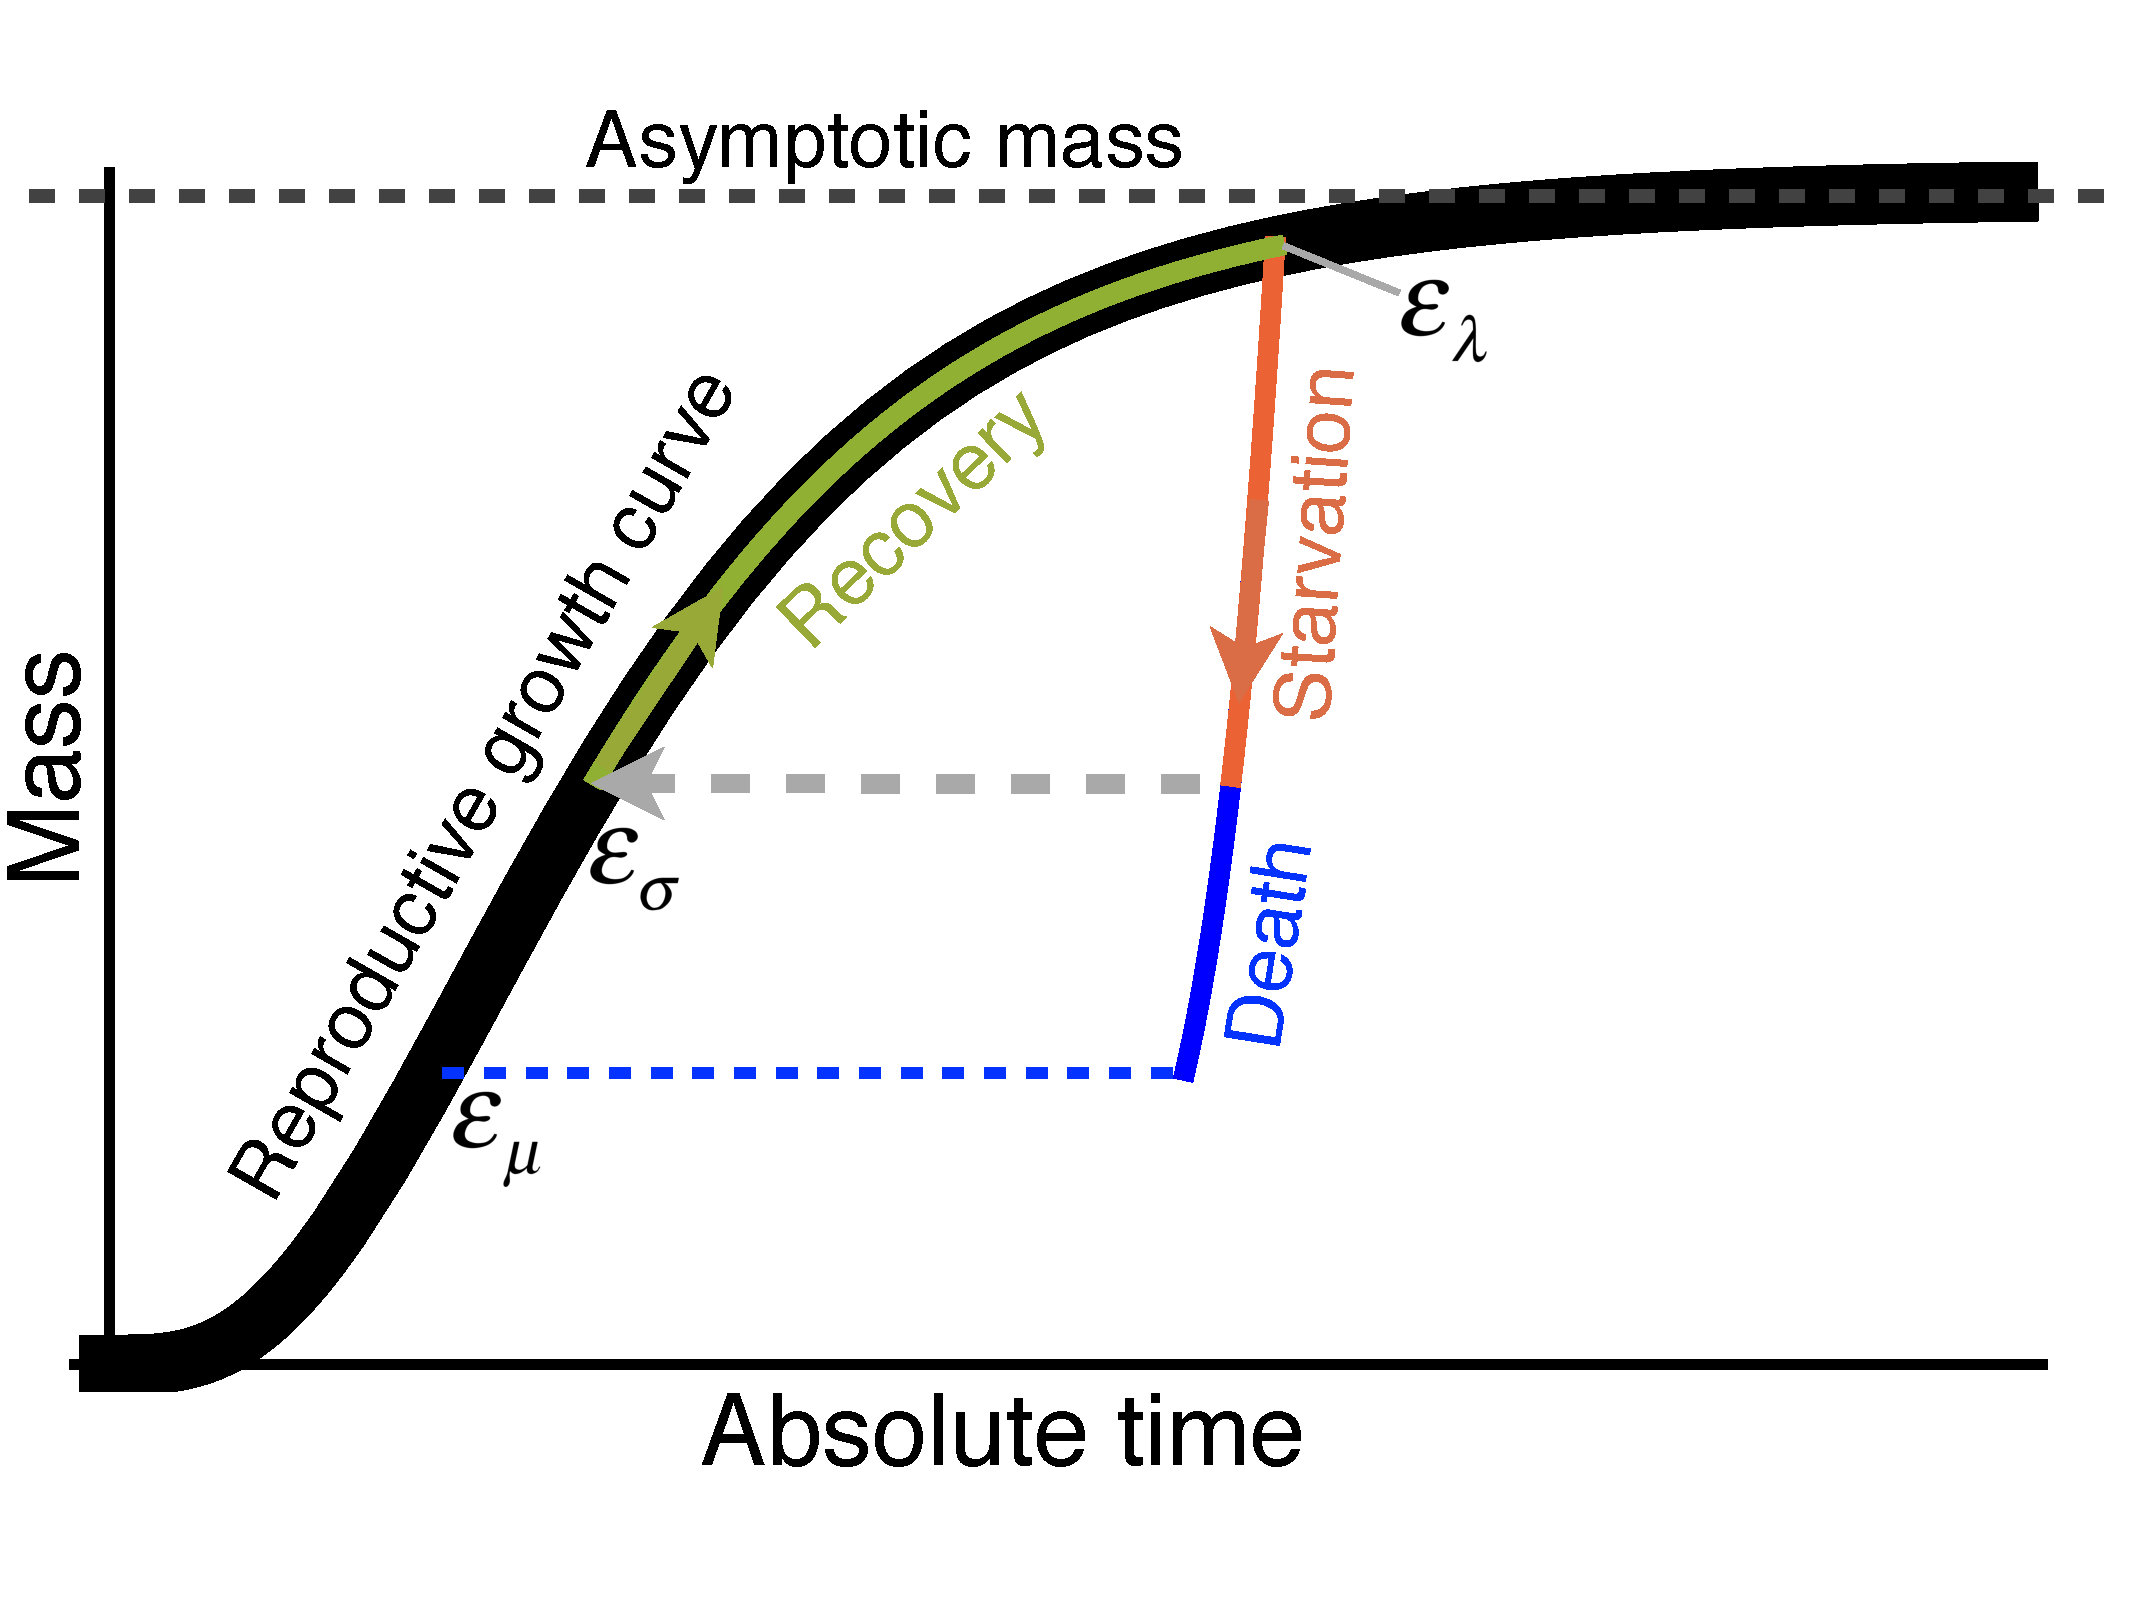
\includegraphics[width=0.375\textwidth]{Growth-trajectory-diagram.pdf}
\caption{\small The growth trajectory over absolute time of an individual
  organism as a function of body mass.  Initial growth follows the black
  trajectory to an energetically replete reproductive adult mass
  $m=\epsilon_\lambda M$ which we assume is 95\% asymptotic mass $M$.
  Starvation follows the red trajectory to
  $m = \epsilon_\sigma \epsilon_\lambda M$, and recovery follows the green
  growth trajectory to the replete adult mass. Alternatively, death from
  starvation follows the blue trajectory to
  $m=\epsilon_\mu \epsilon_\lambda M$.}
\label{fig:growth}
\end{figure}

Several efforts have shown how a partitioning of $B$ between growth and
maintenance purposes can be used to derive a general equation for both the
growth trajectories and growth rates of organisms ranging from bacteria to
metazoans
\cite{West:2001bv,moses2008rmo,gillooly2002esa,hou,Kempes:2012hy}. This relation is derived from the simple balance condition \cite{West:2001bv,moses2008rmo,gillooly2002esa,hou,Kempes:2012hy}
\begin{eqnarray}
\label{balance}
B_{0}m^{\eta}=E_{m}\dot{m}+B_{m}m\,,
\end{eqnarray}
where $E_{m}$ is the energy needed to synthesize a unit of mass, $B_{m}$ is
the metabolic rate to support an existing unit of mass, and $m$ is the mass
of the organism at any point in its development.  This balance has the
general solution \cite{bettencourt,Kempes:2012hy}
\begin{eqnarray}
\label{m1}
\left(\frac{m\left(t\right)}{M}\right)^{1-\eta}\!=1\!-\!\left[1\!-\!\left(\frac{m_{0}}{M}\right)^{1\!-\!\eta}\right]e^{-a\left(1\!-\!\eta\right)t/M^{1-\eta}}
\end{eqnarray}
where, for $\eta<1$, $M=(B_{0}/B_{m})^{1/(1-\eta)}$ is the asymptotic mass,
$a=B_{0}/E_{m}$, and $m_0$ is mass at birth.  We now use this solution to
define the timescale of reproduction and recovery from starvation
(Fig.~\ref{fig:growth}; see \cite{moses2008rmo} for a detailed presentation
of these timescales). The time that it takes to reach a particular mass
$\epsilon M$ is given by the timescale
\begin{equation}
\label{t1}
\tau\left(\epsilon\right) = \ln\left[\frac{1-\left(m_{0}/M\right)^{1-\eta}}{1-\epsilon^{1-\eta}}\right]\frac{M^{1-\eta}}{a\left(1-\eta\right)}
\end{equation}
where we will define values of $\epsilon$ to describe a set of rates within
our model. For the time to reproduce,
$t_{\lambda}=\tau\left(\epsilon_{\lambda}\right)$, where $\epsilon_{\lambda}$
is the fraction of the asymptotic mass where an organism is reproductively
mature and should be close to one (typically $\epsilon_{\lambda}\approx0.95$
\cite{West:2001bv}). The growth rate is then given by
$\lambda=\ln\left(\upsilon\right)/t_{\lambda}$ where $\upsilon$ is the number
of offspring produced, and for any constant value of $\epsilon_{\lambda}$
this will scale like $\lambda\propto M^{\eta-1}$ for $M>>m_{0}$
\cite{West:2001bv,moses2008rmo,gillooly2002esa,hou,Kempes:2012hy}.


\begin{figure}[ht]
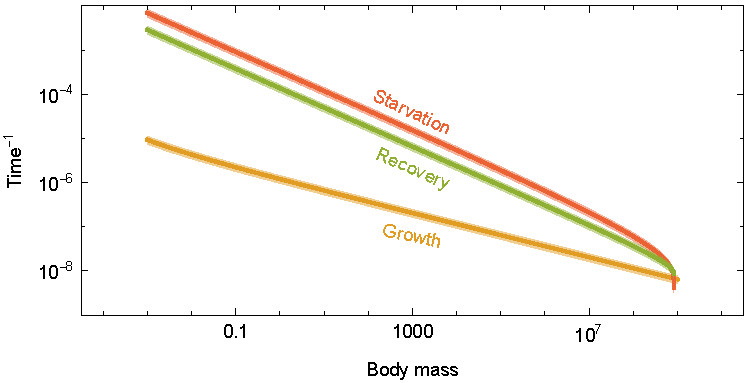
\includegraphics[width=0.45\textwidth]{fig_Rates.pdf}
\caption{\small Allometrically constrained starvation rate $\sigma$ (red) and
  recovery rate $\rho$ (green) relative to the reproductive rate $\lambda$
  (orange) as a function of body mass.  The rate of starvation is greater
  than the rate of reproduction for all realized terrestrial endotherm body
  sizes.  Mean values $\pm 20\%$ variation are shown by the shaded region for
  each rate.  }
\label{fig:gvs}
\end{figure}


The rate of recovery $\rho = 1/t_\rho$ requires that an organism accrues
sufficient tissue to transition from the hungry to the full state.  Since
only certain tissues can be digested for energy (for example the brain cannot
be degraded to fuel metabolism), we define the rates for starvation, death,
and recovery by the timescales required to reach, or return from, specific
fractions of the replete-state mass (Fig. \ref{fig:gvs}; see Supporting
Information, Table I for parameterizations).  We define
$m_{\sigma}=\epsilon_{\sigma} M$, where $\epsilon_{\sigma}<1$ is the fraction
of replete-state mass where reproduction ceases. This fraction will be
modified if tissue composition systematically scales with adult mass.  For
example, making use of the observation that body fat in mammals scales with
overall body size according to $M_{\rm fat}=f_{0}M^{\gamma}$ and assuming
that once this mass is fully digested the organism starves, this would imply
that $\epsilon_{\sigma}=1-f_{0}M^{\gamma}/M$. It follows that the recovery
timescale, $t_{\rho}$, is the time to go from
$m=\epsilon_{\sigma} \epsilon_{\lambda} M$ to $m=\epsilon_{\lambda}M$
(Fig. \ref{fig:growth}). Using Eqs.~\eqref{m1} and \eqref{t1} this timescale
is given by simply considering an adjusted starting mass of
$m_{0}^{\prime}=\epsilon_{\sigma}\epsilon_{\lambda}M$, in which case
\begin{eqnarray}
t_{\rho}=\ln\left[\frac{1-\left(\epsilon_{\sigma}\epsilon_{\lambda}\right)^{1-\eta}}{1-\epsilon^{1-\eta}}\right]\frac{M^{1-\eta}}{a^{\prime}\left(1-\eta\right)}
\end{eqnarray}
where $a^{\prime}=B_{0}/E_{m}^{\prime}$ accounts for possible deviations in the biosynthetic energetics during recovery (see Supporting Information). It should be noted that more complicated ontogenetic models explicitly handle
storage \cite{hou}, whereas this feature is implicitly covered by the body
fat scaling in our framework.

To determine the starvation rate, $\sigma$, we are interested in the time
required for an organism to go from a mature adult that reproduces at rate
$\lambda$, to a
reduced-mass hungry state where reproduction is impossible.  For starving individuals we assume that an organism must meet its maintenance requirements using the digestion of existing mass as the sole energy source.
This assumption implies the following simple metabolic balance 
\begin{eqnarray}
\dot{m}E_{m}^{\prime}=-B_{m}m
\end{eqnarray}
or
\begin{eqnarray}
\dot{m}=-\frac{a^{\prime}}{M^{1-\eta}}m
\end{eqnarray}
where $E_{m}^{\prime}$ is the amount of energy stored in a unit of existing
body mass which differs from $E_{m}$, the energy required to
synthesis a unit of biomass \cite{hou}. Given the replete mass, $M$, of an organism, the
above energy balance prescribes the mass trajectory of a non-consuming
organism:
\begin{eqnarray}
\label{mt}
m\left(t\right)=Me^{-a^{\prime}t/M^{1-\eta}}.
\end{eqnarray}
The time scale for starvation is
given by the time it takes $m(t)$ to reach $\epsilon_{\sigma} M$, which gives
\begin{equation}
\label{eq:sigma}
t_{\sigma}=-\frac{M^{1-\eta}}{a^{\prime}}\ln\left(\epsilon_{\sigma}\right).
\end{equation}
The starvation rate is then $\sigma=1/t_{\sigma}$, which scales with
replete-state mass as $1/M^{1-\eta}\ln\left(1-f_{0}M^{\gamma}/M\right)$.  An important
feature is that $\sigma$ does not have a simple scaling dependence on
$\lambda$ (Fig.~\ref{fig:gvs}), which is important for the dynamics that we
later discuss.

The time to death should follow a similar relation, but defined by a lower
fraction of replete-state mass, $m_{\mu}=\epsilon_{\mu} M$.
Suppose, for example, that an organism dies once it has digested all fat and
muscle tissues, and that muscle tissue scales with body mass according to
$M_{\rm musc}=u_{0}M^{\zeta}$.  This gives
$\epsilon_{\mu}=1-\left(f_{0}M^{\gamma}+u_{0}M^{\zeta}\right)/M$. Muscle
mass has been shown to be roughly proportional to body mass~\cite{Folland:2008ij} in
mammals and thus $\epsilon_{\mu}$ is merely $\epsilon_{\sigma}$ minus a constant. The time to death is the total time to reach $\epsilon_{\mu}M$ minus the time to starve, or
\begin{eqnarray}
t_{\mu}=-\frac{M^{1-\eta}}{a^{\prime}}\ln\left(\epsilon_{\mu}\right)-t_{\sigma},
\end{eqnarray}
and $\mu=1/t_{\mu}$. 


Although the rate equations \eqref{eq:system} are general, here we focus on
parameterizations for terrestrial-bound endotherms, specifically mammals,
which range from a minimum of $M\approx1$g (the Etruscan shrew
\emph{Suncus etruscus}) to a maximum of $M\approx10^7$g (the late Eocene
to early Miocene Indricotheriinae).  Investigating other classes of organisms
would simply involve altering the metabolic exponents and scalings associate
with $\epsilon$. Moreover, we emphasize that our allometric equations
describe mean relationships, and do not account for the (sometimes
considerable) variance associated with individual species.


\section*{Stabilizing effects of allometric constraints}
As the allometric derivations of the NSM rate laws reveal, starvation and recovery rates are not independent parameters, and the biologically relevant portion of the phase space shown in Fig.~\ref{fig:fp} is constrained via covarying parameters.  
Given the parameters of terrestrial endotherms, we find that the starvation rate $\sigma$ and the recovery rate $\rho$ are constrained to lie within a small window of potential values (Fig.~\ref{fig:hopf}) for the known range of body sizes $M$. 
We thus find that the dynamics for all mammalian body sizes is confined to the steady-state regime of the NSM and that limit-cycle behavior is precluded.
Moreover, for larger $M$, the distance to the Hopf bifurcation increases, while uncertainty in allometric parameters (20\% variation around the mean; Fig.~\ref{fig:hopf}) results in little qualitative difference in the distance to the the Hopf bifurcation. 
These results suggest that small mammals are more prone to population oscillations---both stable limit cycles and transient cycles---than mammals with larger body size.  
Thus our NSM model predicts that population cycles should be less common for larger species and more common for smaller species, particularly in environments where resources are limiting.

\begin{figure}
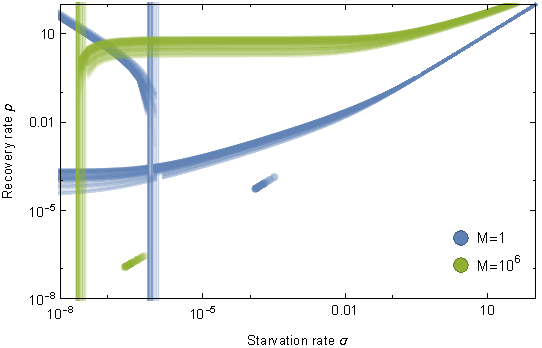
\includegraphics[width=0.425\textwidth]{fig_DataHopf.pdf}
\caption{\small Transcritical (vertical lines) and Hopf bifurcations (curves) for
  allometrically determined starvation $\sigma$ and recovery $\rho$ rates as
  a function of different mammalian body sizes: $M=A\times10^1$g (blue) and
  $M=A\times10^6$g (green), where $A$ is a random uniform variable in $[1,9]$.
  Points denote realized values of $\sigma$ and $\rho$ given the drawn values for $M$.
  }
\label{fig:hopf}
\end{figure}

It should be noted that previous studies have used allometric constraints to
explain the periodicity of cyclic populations
\cite{CalderIII:1983jd,Peterson:1984hj,Krukonis:1991fk}, suggesting a period
$\propto M^{0.25}$.  However this relation seems to hold only for some
species \cite{Hendriks:2012fc}, and potential drivers range from predator
and/or prey lifespans to competitive
dynamics~\cite{Kendall:1999iy,Hogstedt:2005cr}.  Statistically significant
support for the existence of population cycles among mammals is predominantly
based on time series for small mammals~\cite{Kendall:1998hl}, in agreement
with our predictions of more pronounced transient dynamics, given how close
these points are to the Hopf bifurcation.  On the other hand, the longer
gestational times and the increased difficulty in measurements, precludes
obtaining similar-quality data for larger organisms.  

\section*{Extinction risk}
Within our model, higher rates of starvation result in a larger flux of the
population to the hungry state.  In this state reproduction is absent, thus
increasing the likelihood of extinction.  From the perspective of population
survival, it is the rate of starvation relative to the rate of recovery that
determines the long-term dynamics of the various species (Fig.~\ref{fig:fp}).
We therefore examine the competing effects of cyclic dynamics vs.\ changes in
steady state density on extinction risk as a function of $\sigma$ and $\rho$.
To this end, we computed the probability of extinction, where we define
extinction as a population trajectory falling below one tenth of the
allometrically constrained steady state at any time between $t=10^5$ and
$t \leq 10^8$.  This procedure is repeated for 1000 replicates of the
continuous-time system shown in Eq.~\ref{eq:system} for an organism of
$M=100$ grams.  In each replicate the initial densities are chosen to be
$A(F^*,H^*,R^*)$, with $A$ a random variable that is uniformly distributed in
$[0,2]$.  By allowing the rate of starvation to vary, we assessed extinction
risk across a range of values for $\sigma$ and $\rho$ between ca.\ $10^{-6}$
to $10^{-1}$.  As expected, higher rates of extinction correlate with both
high values of $\sigma$ if $\rho$ is small, and high values of $\rho$ if
$\sigma$ is small.  For low values of $\sigma$ and high values of $\rho$, the
increased extinction risk results from transient cycles with larger
amplitudes as the system nears the Hopf bifurcation (Fig.~\ref{fig:ext}).
For high values of $\sigma$ and low values of $\rho$, higher extinction risk
arises because of the decrease in the steady state consumer population
density (Figs.~\ref{fig:fp}\emph{B}, \ref{fig:ext}).  This interplay creates
an `extinction refuge', such that for a constrained range of $\sigma$ and
$\rho$, extinction probabilities are minimized.


\begin{figure}
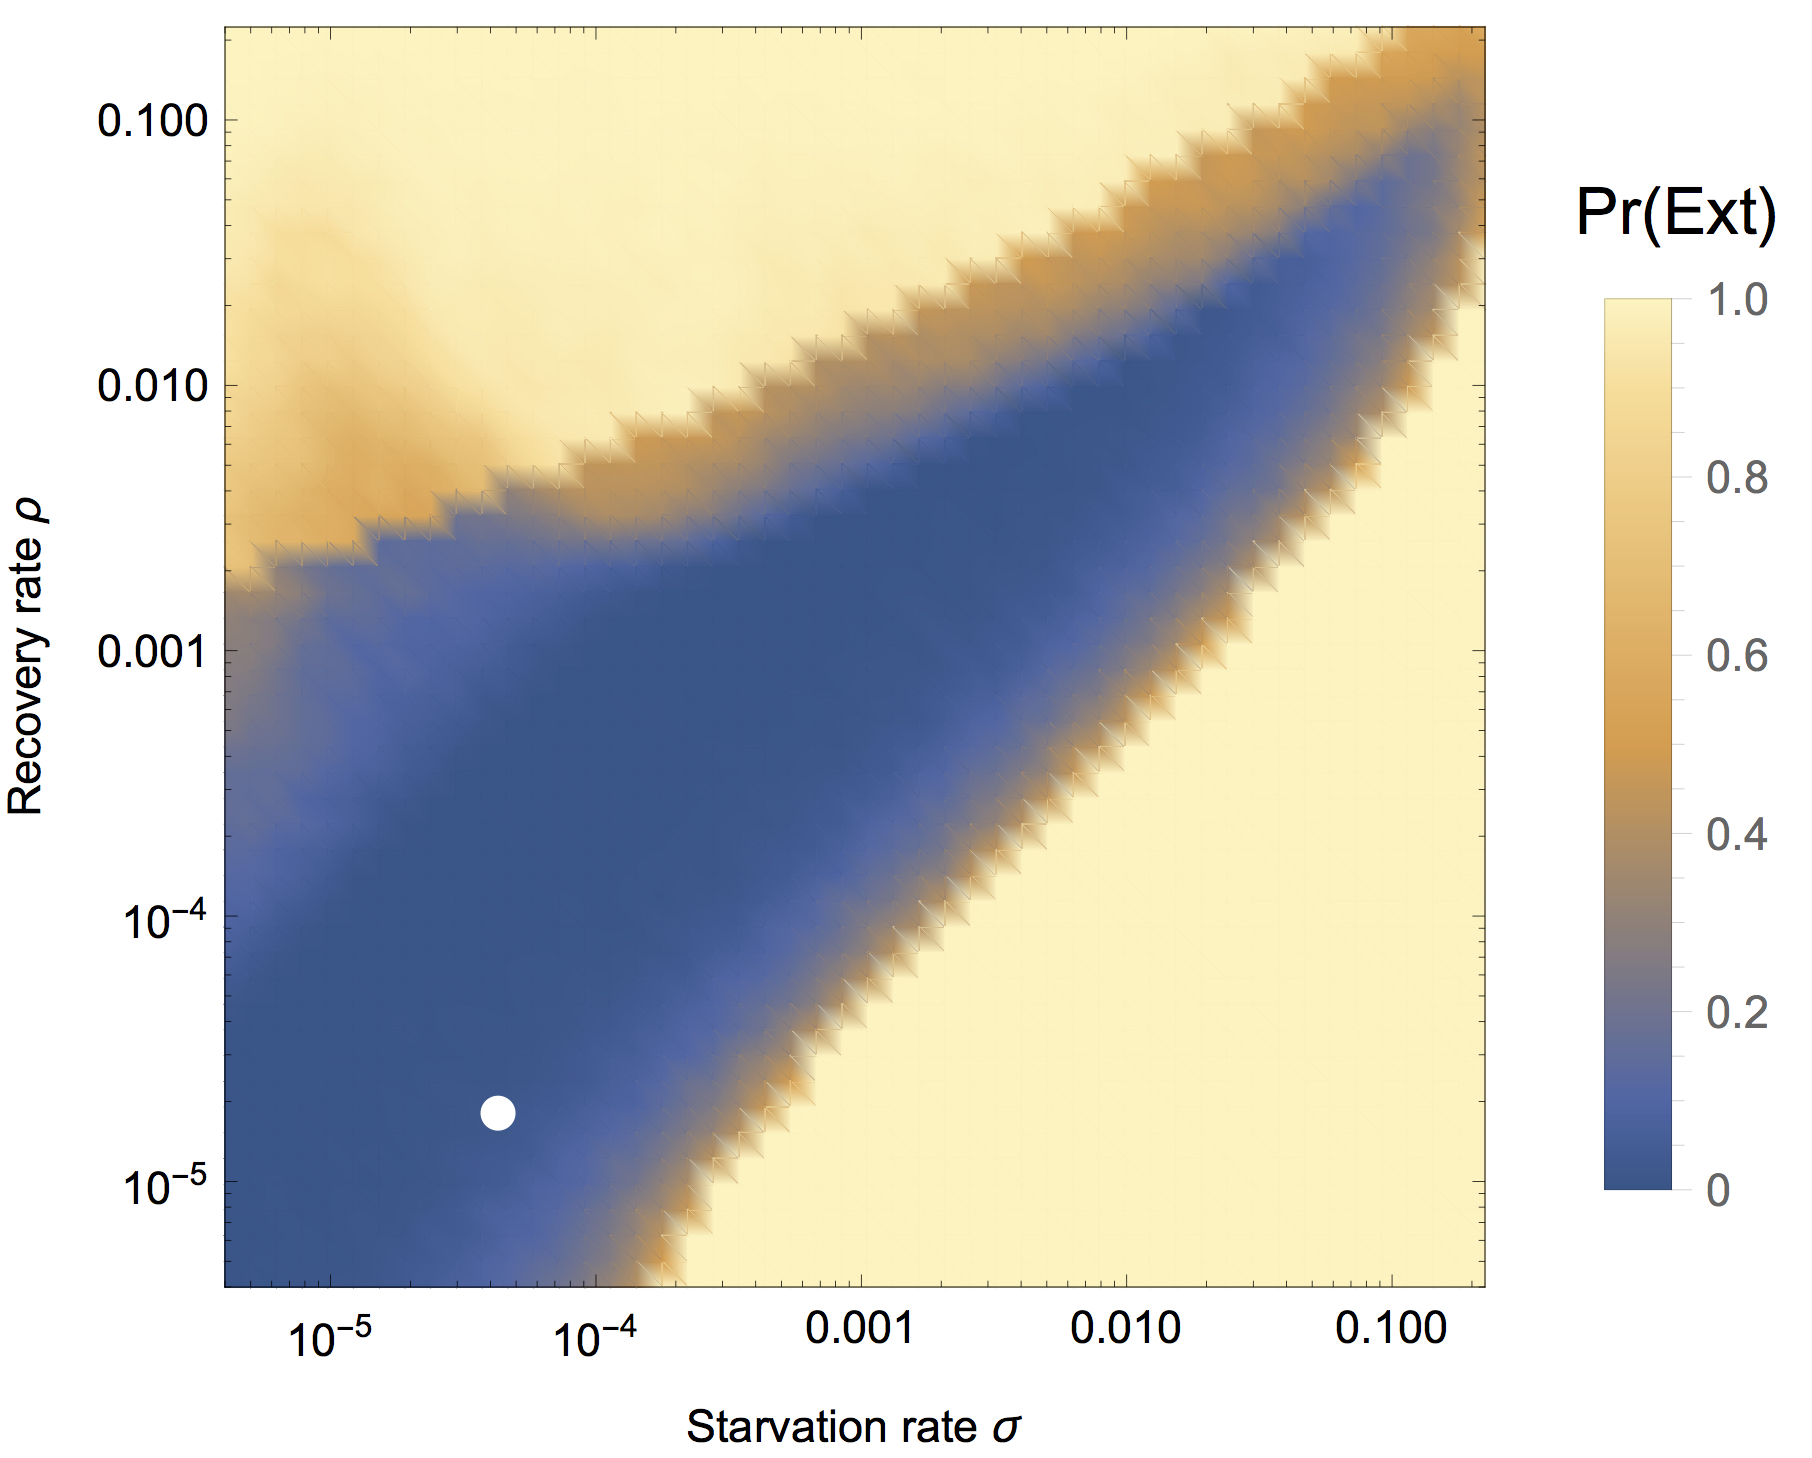
\includegraphics[width=0.425\textwidth]{fig_ExtinctionAllometric.jpg}
\caption{\small Probability of extinction for a 100g consumer as a function of the
  starvation rate $\sigma$ and recovery rate $\rho$, where the initial
  density is given as $A(F^*,H^*,R^*)$, with $A$ being a random uniform
  variable in $[0,2]$.  Extinction is defined as the population trajectory
  falling below $0.1~\times$ the allometrically constrained steady state. The
  white point denotes the allometrically constrained starvation and recovery
  rate.}
\label{fig:ext}
\end{figure} 

We find that the allometrically constrained values of $\sigma$ and $\rho$
fall squarely within the extinction refuge (Fig. \ref{fig:ext}, white point).
These values are close enough to the Hopf bifurcation to avoid low steady
state densities, and far enough away to avoid large-amplitude transient
cycles.  The fact that allometric values of $\sigma$ and $\rho$ fall within
this relatively small window supports the possibility that a selective
mechanism has constrained the physiological conditions that drive starvation
and recovery rates within populations.  Such a mechanism would select for
organism physiology that generates appropriate $\sigma$ and $\rho$ values
that serve to minimize extinction risk.  This selection could occur via the
tuning of body fat percentages, metabolic rates, and biomass maintenance
efficiencies.  To summarize, our finding that the allometrically-determined
parameters fall within this low extinction probability region suggests that
the NSM dynamics may both drive---and constrain---natural animal populations.

\section*{Dynamic and energetic barriers to body size}
Metabolite transport constraints are widely thought to place strict
boundaries on biological
scaling~\cite{Brown:1993p708,West:1997cg,Brown:2004wq} and thereby lead to
specific predictions on the minimum possible body size for
organisms~\cite{West:2002ud}.  Above this bound, a number of energetic and
evolutionary mechanisms have been explored to assess the costs and benefits
associated with larger body masses, particularly for mammals.  One important
such example is the \emph{fasting endurance hypothesis}, which contends that
larger body size, with consequent lower metabolic rates and increased ability
to maintain more endogenous energetic reserves, may buffer organisms against
environmental fluctuations in resource availability~\cite{Millar:1990p923}.
Over evolutionary time, terrestrial mammalian lineages show a significant
trend towards larger body size (known as Cope's
rule)~\cite{Alroy:1998p1594,Clauset:2009fh,Smith:2010p3442,Saarinen:2014br},
and it is thought that within-lineage drivers generate selection towards an
optimal upper bound of roughly $10^7$ grams~\cite{Alroy:1998p1594}, a value
that is likely limited by higher extinction risk for large taxa over longer
timescales~\cite{Clauset:2009fh}.  These trends are thought to be driven by a
combination of climate change and niche availability~\cite{Saarinen:2014br};
however the underpinning energetic costs and benefits of larger body sizes,
and how they influence dynamics over ecological timescales, have not been
explored.  We argue that the NSM provides a suitable framework to explore
these issues.


 
\begin{figure}
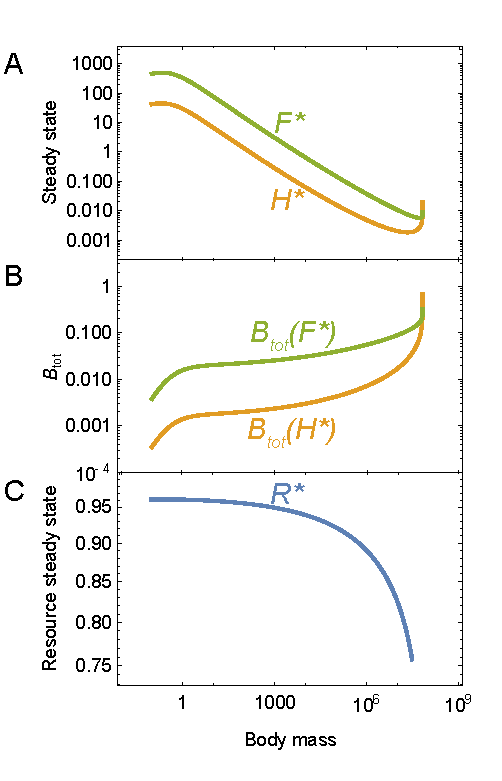
\includegraphics[width=0.4\textwidth]{fig_FPAllometric.pdf}
\caption{\small (\emph{A}) Consumer steady states $F^*$ (green) and $H^*$
  (orange) as a function of body mass.  (\emph{B}) Total energetic use
  $B_{\rm tot}$ of consumer populations at the steady state as a function of
  body mass.  (\emph{C}) Resource steady state $R^*$ as a function of
  consumer body mass.}
\label{fig:mass}
\end{figure}  

The NSM correctly predicts that species with smaller masses have larger
steady-state population densities (Fig.~\ref{fig:mass}\emph{A}).  Moreover,
we show that the NSM provides independent theoretical support for the energy
equivalence hypothesis \cite{allen2002,enquist1998}.  The energy equivalence
hypothesis argues that the total energy use, $B_{tot}$, of a population is
constant independent of species size (e.g.
\cite{allen2002,enquist1998}). %Previous studies have focused on t
This hypothesis is based on observations showing that the abundance, $N$, of
a species is proportional to the inverse of individual metabolism
(e.g. $N\propto M^{-3/4}/B_{0}$) (e.g. \cite{allen2002,enquist1998}).  This
is usually stated as $B_{tot}=NB=C$ where $C$ is a constant, and has been
shown to hold in both mammalian and vascular plant communities
\cite{allen2002,enquist1998}.  Figure \ref{fig:mass}\emph{A} shows that both
$F^{*}$ and $H^{*}$ scale like $M^{-\eta}$ over a wide range of organism
sizes and Figure \ref{fig:mass}\emph{B} shows that $F^{*}B$ is relatively
constant over this same range.  This result if remarkable because it
illustrates that the steady state values of the NSM combined with the derived
timescales naturally give rise to the energy equivalence result.  Our model
shows that the equivalence breaks down at both the minimum and maximum
observed body sizes for mammals, suggesting that these are hard limits where
deviations outside of this range are energetically suboptimal.  Significant
deviations from constant energy use occur at $M \lesssim 1$ at the small end
of the mammalian range and $M\approx 6.5*10^7$ at the large end.


We contend that the NSM provides a mechanistic understanding of the energetic
dynamics that give rise to both observed limitations on mammalian body size
as well as the observed trend towards larger body size over evolutionary
time.  The NSM predicts that the steady state resource density $R^{*}$
decreases with increasing body size of the consumer population
(Fig. \ref{fig:mass}\emph{C}), and classic resource competition theory
predicts that the species surviving on the lowest resource abundance will
outcompete others \cite{tilman1981,dutkiewicz2009,barton2010}.  Thus, the
combined NSM steady-state dynamics and allometric timescales predict that
larger mammals have an intrinsic competitive advantage given a common
resource, but does not offer a within-lineage mechanism by which larger body
sizes are selected for.

To examine whether the NSM could provide such a mechanism, we begin by noting
that a theoretical upper bound on mammalian body size is given by
$\epsilon_\sigma=0$, where mammals are entirely composed of metabolic
reserves, and this occurs at $M=8.3\times 10^8$, or $4.5\times$ the mass of a
blue whale.  Next we examine to what extent a more realistic upper bound to
body mass may serve as an evolutionary attractor, thus providing a suitable
within-lineage mechanism for Cope's rule.  We directly assess the
susceptibility of an otherwise homogeneous population to invasion by a
mutated subset of the population (denoted by ${}^\prime$) where individuals
have a modified proportion of body fat $M^\prime=M(1+\chi)$ where
$\chi \in [-1,1]$, thus altering the rates of starvation $\sigma(M^\prime)$,
recovery $\rho(M^\prime)$, and maintenance $\beta(M^\prime)$.  There is no
internal fixed point corresponding to a state where both original residents
and invaders coexist (except for the trivial state $\chi=0$).  To assess the
susceptibility to invasion as a function of the invader mass, we determine
which consumer has a higher steady-state density for a given value of $\chi$.
We find that for $1\leq M<8.43\times 10^6$g, having additional body fat
($\chi > 0$) results in a higher steady-state invader population density
($H^{\prime *}+F^{\prime *}>H^*+F^*$).  Thus the invader has an intrinsic
advantage over the resident population.  However, for $M>8.43\times 10^6$,
leaner individuals ($\chi < 0$) have advantageous steady state densities
(Fig.~\ref{fig:invasion}).


\begin{figure}
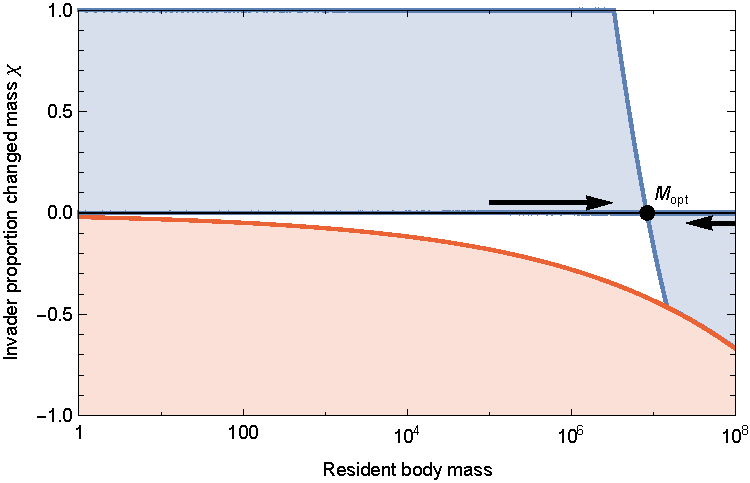
\includegraphics[width=0.45\textwidth]{fig_Invasion.pdf}
\caption{\small Invasion feasibility for organisms with a proportional change
  in mass $\chi$ against a population with a resident body mass $M$.  The
  blue region denotes proportions of modified mass $\chi$ resulting in
  successful invasion.  The red region denotes values of $\chi$ that result
  in a mass that is below the starvation threshold and is thus infeasible.
  Arrows point to the predicted optimal mass $M_{\rm opt}=8.43\times 10^6$,
  which serves as the uninvadable, evolutionary stable state.}
\label{fig:invasion}
\end{figure}  
 

The observed switch in susceptibility as a function of $\chi$ at
$M_{\rm opt}=8.43 \times 10^6$ thus serves as an attractor, or an uninvadable
evolutionary stable state, such that the NSM predicts organismal mass to
increase if $M<M_{\rm opt}$ and decrease if $M>M_{\rm opt}$.  Moreover,
$M_{\rm opt}$, which is entirely determined by the population-level
consequences of energetic constraints, is remarkably close to the maximum
body size observed in the North American mammalian fossil
record~\cite{Alroy:1998p1594} as well as the mass predicted from an
evolutionary model of body size evolution~\cite{Clauset:2009fh}.  While the
state of the environment, as well as the competitive landscape, will
determine whether specific body sizes are selected for or
against~\cite{Saarinen:2014br}, we suggest that the dynamics of starvation
and recovery described in the NSM may provide a general driving mechanism for
the evolution of larger body size among terrestrial mammals.


%Closing
The energetics associated with somatic maintenance, growth, and reproduction
are important elements that influence the dynamics of all
populations~\cite{Stearns:1989ip}.  The NSM is a minimal and general model
that incorporates the dynamics of starvation and recovery that are expected
to occur in resource-limited environments.  By incorporating allometric
relations between the rates in the NSM, we found: (i) different organismal
masses have distinct population dynamic regimes, (ii)
allometrically-determined rates of starvation and recovery appear to minimize
extinction risk, and (iii) the dynamic consequences of these rates may
introduce additional drivers and hard boundaries on the evolution of minimum
and maximum body size.  We suggest that the NSM offers a means by which the
dynamic consequences of energetic constraints can be assessed using
macroscale interactions between and among species.  Future efforts will
involve exploring the consequences of these dynamics in a spatially explicit
framework, thus incorporating elements such as movement costs and spatial
heterogeneity, which may elucidate additional tradeoffs associated with the
dynamics of starvation and recovery.

\vspace{2mm}

\noindent {\bf Acknowledgments} {\small We thank Luis Bettencourt, Jean
  Philippe Gibert, Eric Libby, and Seth Newsome for helpful discussions and
  comments on the manuscript.  J.D.Y. was supported by startup funds at the
  University of California, Merced, and an Omidyar Postdoctoral Fellowship at
  the Santa Fe Institute.  C.P.K. was supported by an Omidyar Postdoctoral
  Fellowship at the Santa Fe Institute.  S.R. was supported by grants
  DMR-1608211 and 1623243 from the National Science Foundation, and by the
  John Templeton Foundation, all at the Santa Fe Institute.  }


%\bibliography{aa_starving3}
\small{
\begin{thebibliography}{10}

\bibitem{Martin:1987dl} T.~E. Martin, ``{Food as a Limit on Breeding Birds: A
    Life-History Perspective},'' {\em Annu.\ Rev.\ Ecol.\ Syst.}, vol.~18,
  pp.~453--487, Jan.\ 1987.

\bibitem{Kirk:1997cc} K.~L. Kirk, ``{Life-History Responses to Variable
    Environments: Starvation and Reproduction in Planktonic Rotifers},'' {\em
    Ecology}, vol.~78, pp.~434--441, Mar.\ 1997.

\bibitem{Kempes:2012hy} C.~P. Kempes, S.~Dutkiewicz, and M.~J. Follows,
  ``{Growth, metabolic partitioning, and the size of microorganisms.},'' {\em
    Proc.  Natl. Acad. Sci. USA}, vol.~109, pp.~495--500, Jan.\ 2012.

\bibitem{Mangel:1988uaa} M.~Mangel and C.~W. Clark, {\em {Dynamic Modeling in
      Behavioral Ecology}}.  \newblock Princeton: Princeton University Press,
  1988.

\bibitem{Mangel:2014kz} M.~Mangel, ``{Stochastic dynamic programming
    illuminates the link between environment, physiology, and evolution},''
  {\em Bull.\ Math.\ Biol.}, vol.~77, no.~5, pp.~857--877, 2014.

\bibitem{Yeakel:2013hi} J.~D. Yeakel, N.~J. Dominy, P.~L. Koch, and
  M.~Mangel, ``{Functional morphology, stable isotopes, and human evolution:
    a model of consilience},'' {\em Evolution}, vol.~68, no.~1, pp.~190--203,
  2014.

\bibitem{Morris:1987eo} D.~W. Morris, ``{Optimal Allocation of Parental
    Investment},'' {\em Oikos}, vol.~49, p.~332, July 1987.

\bibitem{Tveraa:2003fq} T.~Tveraa, P.~Fauchald, C.~Henaug, and N.~G. Yoccoz,
  ``{An examination of a compensatory relationship between food limitation
    and predation in semi-domestic reindeer},'' {\em Oecologia}, vol.~137,
  pp.~370--376, Nov.\ 2003.

\bibitem{Daan:1988va} S.~Daan, C.~Dijkstra, R.~Drent, and T.~Meijer, ``{Food
    supply and the annual timing of avian reproduction},'' in {\em
    Proceedings of the International Ornithological Congress} vol.~19,
    pp.~392-407, 1988.

\bibitem{Jacot:2009dv} A.~Jacot, M.~Valcu, K.~van Oers, and B.~Kempenaers,
  ``{Experimental nest site limitation affects reproductive strategies and
    parental investment in a hole-nesting passerine},'' {\em Animal
    Behaviour}, vol.~77, pp.~1075--1083, May 2009.

\bibitem{Stearns:1989ip} S.~C. Stearns, ``{Trade-Offs in Life-History
    Evolution},'' {\em Funct. Ecol.}, vol.~3, no.~3, p.~259, 1989.

\bibitem{Barboza:2002in} P.~Barboza and D.~Jorde, ``{Intermittent fasting
    during winter and spring affects body composition and reproduction of a
    migratory duck},'' {\em J. Comp.\ Physiol.\ B}, vol.~172, pp.~419--434,
  July 2002.

\bibitem{Threlkeld:1976ih} S.~T. Threlkeld, ``{Starvation and the size
    structure of zooplankton communities},'' {\em Freshwater Biol.}, vol.~6,
  pp.~489--496, Dec.\ 1976.

\bibitem{Weber:1998jg} T.~P. Weber, B.~J. Ens, and A.~I. Houston, ``{Optimal
    avian migration: A dynamic model of fuel stores and site use},'' {\em
    Evolutionary Ecology}, vol.~12, pp.~377--401, May 1998.

\bibitem{Mduma:1999cp} S.~A.~R. Mduma, A.~R.~E. Sinclair, and R.~Hilborn,
  ``{Food regulates the Serengeti wildebeest: a 40-year record},'' {\em
    J. Anim.\ Ecol.}, vol.~68, pp.~1101--1122, Nov.\ 1999.

\bibitem{Moore:2014hi} J.~W. Moore, J.~D. Yeakel, D.~Peard, J.~Lough, and
  M.~Beere, ``{Life-history diversity and its importance to population
    stability and persistence of a migratory fish: steelhead in two large
    North American watersheds},'' {\em J.  Anim.\ Ecol.}, vol.~83, no.~5,
  pp.~1035--1046, 2014.

\bibitem{Mead:1989dt} R.~A. Mead, ``{The Physiology and Evolution of Delayed
    Implantation in Carnivores},'' in {\em Carnivore Behavior, Ecology, and
    Evolution}, pp.~437--464, Boston, MA: Springer US, 1989.

\bibitem{Sandell:1990kw}
M.~Sandell, ``{The Evolution of Seasonal Delayed Implantation},'' {\em The
  Quarterly Review of Biology}, vol.~65, no.~1, pp.~23--42, 1990.

\bibitem{Bulik:1999eo} C.~M. Bulik, P.~F. Sullivan, J.~L. Fear, A.~Pickering,
  A.~Dawn, and M.~McCullin, ``{Fertility and Reproduction in Women With
    Anorexia Nervosa},'' {\em J. Clin.\ Psychiatry}, vol.~60, pp.~130--135,
  Feb.\ 1999.

\bibitem{Trites:2003cc} A.~W. Trites and C.~P. Donnelly, ``{The decline of
    Steller sea lions Eumetopias jubatus in Alaska: a review of the
    nutritional stress hypothesis},'' {\em Mammal Review}, vol.~33,
  pp.~3--28, Mar.\ 2003.

\bibitem{Glazier:2009hq} D.~S. Glazier, ``{Metabolic level and size scaling
    of rates of respiration and growth in unicellular organisms},'' {\em
    Funct.\ Ecol.}, vol.~23, pp.~963--968, Oct.\ 2009.

\bibitem{Kooi2000} S.~A. L.~M. Kooijman, {\em {Dynamic Energy and Mass
      Budgets in Biological Systems}}.  \newblock 2000.

\bibitem{Sousa:2010ez} T.~Sousa, T.~Domingos, J.~C. Poggiale, and
  S.~A. L.~M. Kooijman, ``{Dynamic energy budget theory restores coherence in
    biology},'' {\em Philos.\ Trans.\ Roy.\ Soc.\ B}, vol.~365,
  pp.~3413--3428, Oct.\ 2010.

\bibitem{Diekmann:2010da} O.~Diekmann and J.~A.~J. Metz, ``{How to lift a
    model for individual behaviour to the population level?},'' {\em Philos.\
    Trans.\ Roy.\ Soc.\ B}, vol.~365, pp.~3523--3530, Nov.\ 2010.

\bibitem{murdoch:2003} W.~W. Murdoch, C.~J. Briggs, and R.~M. Nisbet, {\em
    {Consumer-Resource Dynamics}}.  \newblock Monographs in population
  biology, Princeton University Press, 2003.

\bibitem{Benichou:2014wu} O.~Benichou and S.~Redner, ``{Depletion-Controlled
    Starvation of a Diffusing Forager},'' {\em Phys.\ Rev.\ Lett.}, vol.~113,
  p.~238101, Dec.\ 2014.

\bibitem{Benichou:2016wl} O.~B{\'e}nichou, M.~Chupeau, and S.~Redner, ``{Role
    of Depletion on the Dynamics of a Diffusing Forager},'' J. Phys.\ A:
  Math.\ Theor.\ (in press).

\bibitem{Chupeau:2016jf} M.~Chupeau, O.~B{\'e}nichou, and S.~Redner,
  ``{Universality Classes of Foraging with Resource Renewal},'' {\em
    Phys. Rev. E}, vol.~93, p.~032403, Mar.\ 2016.

\bibitem{murray2011mathematical} J.~D. Murray, {\em {Mathematical Biology:
      I. An Introduction}}, vol.~110 of {\em Interdisciplinary Applied
    Mathematics}.  \newblock Melaka Manipal Medical College (Manipal Campus),
  International Centre for Health Sciences, Madhav Nagar, Manipal, Udupi
  District, Karnataka State, India. nayaksathish@yahoo.com: Springer New
  York, 2011.

\bibitem{Strogatz:2008wo} S.~H. Strogatz, {\em {Nonlinear Dynamics and
      Chaos}}.  \newblock With Applications to Physics, Biology, Chemistry,
  and Engineering, Westview Press, Aug.\ 2008.

\bibitem{GuckHolmes} J.~Guckenheimer and P.~Holmes, {\em {Nonlinear
      oscillations, dynamical systems, and bifurcations of vector fields}}.
  \newblock New York: Springer, 1983.

\bibitem{Gross:2004p2428} T.~Gross and U.~Feudel, ``{Analytical search for
    bifurcation surfaces in parameter space},'' {\em Physica D}, vol.~195,
  no.~3-4, pp.~292--302, 2004.

\bibitem{Hastings:2001jh} A.~Hastings, ``{Transient dynamics and persistence
    of ecological systems},'' {\em Ecol.\ Lett.}, vol.~4, pp.~215--220, May
  2001.

\bibitem{Neubert:1997wk} M.~Neubert and H.~Caswell, ``{Alternatives to
    resilience for measuring the responses of ecological systems to
    perturbations},'' {\em Ecology}, vol.~78, no.~3, pp.~653--665, 1997.

\bibitem{Caswell:2005eo} H.~Caswell and M.~G. Neubert, ``{Reactivity and
    transient dynamics of discrete-time ecological systems},'' {\em Journal
    of Difference Equations and Applications}, vol.~11, pp.~295--310, Apr.\
  2005.

\bibitem{Neubert:2009td} M.~Neubert and H.~Caswell, ``{Detecting
    reactivity},'' {\em Ecology}, 2009.

\bibitem{Yodzis:1992hg} P.~Yodzis and S.~Innes, ``{Body Size and
    Consumer-Resource Dynamics},'' {\em Am.\ Nat.}, vol.~139, no.~6,
  pp.~1151--1175, 1992.

\bibitem{Brown:2004wq} J.~Brown, J.~Gillooly, A.~Allen, V.~Savage, and
  G.~West, ``{Toward a metabolic theory of ecology},'' {\em Ecology},
  vol.~85, no.~7, pp.~1771--1789, 2004.

\bibitem{West:2002it}
G.~B. West, W.~H. Woodruff, and J.~H. Brown, ``{Allometric scaling of metabolic
  rate from molecules and mitochondria to cells and mammals.},'' {\em Proc.\
  Natl.\ Acad.\ Sci.\ USA}, vol.~99 Suppl.\ 1, pp.~2473--2478, Feb.\ 2002.

\bibitem{DeLong:2010dy} J.~P. DeLong, J.~G. Okie, M.~E. Moses, R.~M. Sibly,
  and J.~H. Brown, ``{Shifts in metabolic scaling, production, and efficiency
    across major evolutionary transitions of life.},'' {\em Proc.\ Natl.\
    Acad.\ Sci.\ USA}, vol.~107, pp.~12941--12945, July 2010.

\bibitem{West:2001bv} G.~B. West, J.~H. Brown, and B.~J. Enquist, ``{A
    general model for ontogenetic growth},'' {\em Nature}, vol.~413,
  pp.~628--631, Oct.\ 2001.

\bibitem{moses2008rmo} M.~E. Moses, C.~Hou, W.~H. Woodruff, G.~B. West,
  J.~C. Nekola, W.~Zuo, and J.~H. Brown, ``{Revisiting a Model of Ontogenetic
    Growth: Estimating Model Parameters from Theory and Data},'' {\em
    http://dx.doi.org.proxy.lib.sfu.ca/10.1086/679735}, vol.~171,
  pp.~632--645, May 2008.

\bibitem{gillooly2002esa} J.~F. Gillooly, E.~L. Charnov, G.~B. West,
  V.~M. Savage, and J.~H. Brown, ``{Effects of size and temperature on
    developmental time},'' {\em Nature}, vol.~417, pp.~70--73, May 2002.

\bibitem{hou} C.~Hou, W.~Zuo, M.~E. Moses, W.~H. Woodruff, J.~H. Brown, and
  G.~B. West, ``{Energy Uptake and Allocation During Ontogeny},'' {\em
    Science}, vol.~322, pp.~736--739, Oct.\ 2008.

\bibitem{bettencourt} L.~M.~A. Bettencourt, J.~Lobo, D.~Helbing, C.~Kuhnert,
  and G.~B. West, ``{Growth, innovation, scaling, and the pace of life in
    cities},'' {\em Proc.\ Natl.\ Acad.\ Sci.\ USA}, vol.~104,
  pp.~7301--7306, Apr.\ 2007.

\bibitem{Folland:2008ij} J.~P. Folland, T.~M. Mc~Cauley, and A.~G. Williams,
  ``{Allometric scaling of strength measurements to body size},'' {\em Eur.\
    J. Appl.\ Physiol.}, vol.~102, pp.~739--745, Jan.\ 2008.

\bibitem{CalderIII:1983jd} W.~A. Calder~III, ``{An allometric approach to
    population cycles of mammals},'' {\em J. Theor.\ Biol.}, vol.~100,
  pp.~275--282, Jan.\ 1983.

\bibitem{Peterson:1984hj}
R.~O. Peterson, R.~E. Page, and K.~M. Dodge, ``{Wolves, Moose, and the
  Allometry of Population Cycles},'' {\em Science}, vol.~224, pp.~1350--1352,
  June 1984.

\bibitem{Krukonis:1991fk} G.~Krukonis and W.~M. Schaffer, ``{Population
    cycles in mammals and birds: Does periodicity scale with body size?},''
  {\em J. Theor.\ Biol.}, vol.~148, pp.~469--493, Feb.\ 1991.

\bibitem{Hendriks:2012fc}
A.~J. Hendriks and C.~Mulder, ``{Delayed logistic and
  Rosenzweig{\textendash}MacArthur models with allometric parameter setting
  estimate population cycles at lower trophic levels well},'' {\em Ecological
  Complexity}, vol.~9, pp.~43--54, Feb.\ 2012.

\bibitem{Kendall:1999iy} B.~E. Kendall, C.~J. Briggs, W.~W. Murdoch,
  P.~Turchin, S.~P. Ellner, E.~McCauley, R.~M. Nisbet, and S.~N. Wood, ``{Why
    do populations cycle? A synthesis of statistical and mechanistic modeling
    approaches},'' {\em Ecology}, vol.~80, pp.~1789--1805, Sept.\ 1999.

\bibitem{Hogstedt:2005cr} G.~H{\"o}gstedt, T.~Seldal, and A.~Breistol,
  ``{Period length in cyclic animal populations},'' {\em Ecology}, vol.~86,
  pp.~373--378, Feb.\ 2005.

\bibitem{Kendall:1998hl} Kendall, Prendergast, and Bjornstad, ``{The
    macroecology of population dynamics: taxonomic and biogeographic patterns
    in population cycles},'' {\em Ecol. Lett.}, vol.~1, pp.~160--164,
  Nov.\ 1998.

\bibitem{Brown:1993p708} J.~Brown, P.~Marquet, and M.~Taper, ``{Evolution of
    body size: consequences of an energetic definition of fitness},'' {\em
    Am.\ Nat.}, vol.~142, no.~4, pp.~573--584, 1993.

\bibitem{West:1997cg} G.~B. West, J.~H. Brown, and B.~J. Enquist, ``{A
    General Model for the Origin of Allometric Scaling Laws in Biology},''
  {\em Science}, vol.~276, pp.~122--126, Apr.\ 1997.

\bibitem{West:2002ud} G.~B. West, W.~H. Woodruff, and J.~H. Brown,
  ``{Allometric scaling of metabolic rate from molecules and mitochondria to
    cells and mammals},'' {\em Proc.\ Natl.\ Acad.\ Sci.\ USA}, vol.~99,
  no.~Suppl 1, pp.~2473--2478, 2002.

\bibitem{Millar:1990p923} J.~Millar and G.~Hickling, ``{ Fasting Endurance
    and the Evolution of Mammalian Body Size},'' {\em Funct.\ Ecol.}, vol.~4,
  no.~1, pp.~5--12, 1990.

\bibitem{Alroy:1998p1594} J.~Alroy, ``{Cope's rule and the dynamics of body
    mass evolution in North American fossil mammals},'' {\em Science},
  vol.~280, no.~5364, p.~731, 1998.

\bibitem{Clauset:2009fh} A.~Clauset and S.~Redner, ``{Evolutionary Model of
    Species Body Mass Diversification},'' {\em Phys. Rev. Lett.}, vol.~102,
  p.~038103, Jan.\ 2009.

\bibitem{Smith:2010p3442} F.~Smith, A.~Boyer, J.~Brown, and D.~Costa, ``{The
    Evolution of Maximum Body Size of Terrestrial Mammals},'' {\em Science},
  Jan.\ 2010.

\bibitem{Saarinen:2014br} J.~J. Saarinen, A.~G. Boyer, J.~H. Brown,
  D.~P. Costa, S.~K.~M. Ernest, A.~R.  Evans, M.~Fortelius, J.~L. Gittleman,
  M.~J. Hamilton, L.~E. Harding, K.~Lintulaakso, S.~K. Lyons, J.~G. Okie,
  R.~M. Sibly, P.~R. Stephens, J.~Theodor, M.~D. Uhen, and F.~A. Smith,
  ``{Patterns of maximum body size evolution in Cenozoic land mammals:
    eco-evolutionary processes and abiotic forcing},'' {\em Proc.\
    Biol\. Sci.}, vol.~281, pp.~20132049--20132049, June 2014.

\bibitem{allen2002} A.~P. Allen, J.~H. Brown, and J.~F. Gillooly, ``{Global
    Biodiversity, Biochemical Kinetics, and the Energetic-Equivalence
    Rule},'' {\em Science}, vol.~297, pp.~1545--1548, Aug.\ 2002.

\bibitem{enquist1998} B.~J. Enquist, J.~H. Brown, and G.~B. West,
  ``{Allometric scaling of plant energetics and population density : Abstract
    : Nature},'' {\em Nature}, vol.~395, pp.~163--165, Sept.\ 1998.

\bibitem{tilman1981} D.~Tilman, ``{Tests of Resource Competition Theory Using
    Four Species of Lake Michigan Algae},'' {\em Ecology}, vol.~62,
  pp.~802--815, June 1981.

\bibitem{dutkiewicz2009} S.~Dutkiewicz, M.~J. Follows, and J.~G. Bragg,
  ``{Modeling the coupling of ocean ecology and biogeochemistry},'' {\em
    Global Biogeochem.\ Cycles}, vol.~23, pp.~n/a--n/a, Dec.\ 2009.

\bibitem{barton2010} A.~D. Barton, S.~Dutkiewicz, G.~Flierl, J.~Bragg, and
  M.~J. Follows, ``{Patterns of Diversity in Marine Phytoplankton},'' {\em
    Science}, vol.~327, pp.~1509--1511, Mar.\ 2010.

\end{thebibliography}
}



%\end{multicols}



\clearpage





 
\section*{Supporting Information for ``The dynamics of starvation and recovery''}%: Eco-evolutionary feedbacks}


\subsection*{Parameter Values and Estimates}

Many of the parameter values employed in our model have either been directly measured in previous studies or can be estimated from combining several previous studies. Here we outline previous measurements and simple estimates of the parameters. 

\subsubsection*{Standard synthesis and metabolic parameters}

Metabolic rate has been generally reported to follow an exponent close to
$\eta=0.75$ (e.g. \cite{supp:West:2001bv,supp:moses2008rmo} and the
supplement of \cite{supp:hou}). We make this assumption in the current paper,
although alternate exponents, which are know to vary between roughly $0.25$
and $1.5$ for single species \cite{supp:moses2008rmo}, could be easily
incorporated into our framework, and this variation is effectively handled by
the $20\%$ variations that we consider around mean trends. It is important to
note the exponent, because it not only defines several scalings in our
framework but also the value of the metabolic normalization constant,
$B_{0}$, given a set of data.  For mammals the metabolic normalization
constant has been reported to vary between $0.018$ (W g$^{-0.75}$) and
$0.047$ (W g$^{-0.75}$) \cite{supp:hou,supp:West:2001bv}, where the former value
represents basal metabolic rate and the latter represents the field metabolic
rate. We employ the field metabolic rate for our NSM model which is
appropriate for active mammals (Table 1).

The energy to synthesize a unit of biomass, $E_{m}$, has been reported to
vary between $1800$ to $9500$ (J g$^{-1}$)
(e.g. \cite{supp:West:2001bv,supp:moses2008rmo,hou}) in mammals with a mean
value across many taxonomic groups of $5,774$ (J g$^{-1}$)
\cite{supp:moses2008rmo}. The unit energy available during starvation,
$E^{\prime}$, could range between $7000$ (J g$^{-1}$), the return of the
total energy stored during ontogeny \cite{hou} to a biochemical upper bound
of $E^{\prime}=36,000$ (J g$^{-1}$) for the energetics of palmitate
\cite{supp:stryer,supp:hou}. For our calculations we use the measured value
for bulk tissues of $7000$ which assumes that the energy stored during
ontogeny is returned during starvation \cite{supp:hou}.

For the scaling of body composition it has been shown that fat mass follows
$M_{\rm fat}=f_{0}M^{\gamma}$, with measured relationships following
$0.018M^{1.25}$ \cite{supp:Dunbrack:1993ec}, $0.02M^{1.19}$
\cite{supp:Lindstedt:1985hm}, and $0.026M^{1.14}$
\cite{supp:Lindstedt:2002td}. We use the values from
\cite{supp:Lindstedt:1985hm} which falls in the middle of this
range. Similarly, the muscle mass follows $M_{\rm musc}=u_{0}M^{\zeta}$ with
$u_{0}=0.383$ and $\zeta=1.00$ \cite{supp:Lindstedt:2002td}.

The final parameters that we must consider connect the resource growth rate
to the total metabolic rate of an organism. That is, we are interested in the
relative rates of resource recovery and consumption by the total
population. From \cite{supp:allen2002global} the total resource use of a
population with an individual body size of $M$ is given by
$B_{pop}=0.00061x^{-0.03}$ (W m$^{-2}$). Considering an energy density of
$18200$ (J g$^{-1}$) of grass \cite{supp:estermann} and an NPP between and
$1.59\times10^{-6}$ and $7.92\times10^{-5}$ (g s$^{-1}$ m$^{-2}$) would give
a range of resource rates between $0.029$ and $1.44$ (W m$^{-2}$). This gives
a ratio of total resource consumption to supply rates between $0.00042$ and
$0.021$, and we used a value of $0.002$ in our calculations and simulations.

%For the growth rate $\lambda$ we consider the standard model of $\ln\left(\upsilon\right)/t_{\lambda}$

%More complicated models of fecundity (which, for example, account for the average length of adulthood and the number of individuals produced over this span) could be employed. However, the scaling of population growth rate has been studied in detail before and follows a relationship of $$ which matches the theory well for $\phi=.95$ and $=$.

%In our calculations we include $20\%$ variation around this value which could account for differences in efficiency during 

 \begin{table}[h]
\caption{Parameter values for mammals}
\label{param}
    \begin{center}
    \small
     \begin{tabular}{ p{1.8cm} p{2.6cm} l p{2.2cm}|}
     \hline
     Parameter & Value & References  \\
     \hline
   $\eta$ & $3/4$  &  (e.g. \cite{supp:West:2001bv,supp:moses2008rmo,hou}) \\ 
   $E_{m}$ & $5774$ (J gram$^{-1}$)  &  \cite{supp:moses2008rmo,supp:West:2001bv,supp:hou} \\ 
   $E_{m}^{\prime}$ & $36,000$  & \cite{supp:stryer,supp:hou} \\ 
   $B_{0}$ & $0.047$ (W g$^{-0.75}$)    & \cite{supp:hou}  \\
%   $a$ & $1.78\times10^{-6}$  \quad \quad \\ 
%   $\lambda_{0}$ & $3.39\times10^{-7}$ (s$^{-1}$ gram$^{1-\eta}$) \quad \quad \\ 
   $\gamma$ & $1.19$ & \cite{supp:Lindstedt:1985hm} \\ 
   $f_{0}$ & $0.02$ & \cite{supp:Lindstedt:1985hm}\\ 
   $\zeta$ & $1.00$  & \cite{supp:Lindstedt:2002td} \\ 
   $u_{0}$ & $0.38$  & \cite{supp:Lindstedt:2002td} \\ 
      
   \hline
    \end{tabular}
    \end{center}
   \end{table}


\subsubsection*{Rate equations for invaders with modified body mass}
If an invading subset of the resident population of mass $M$ has an altered
mass $M^\prime = M(1+\chi)$ where $\chi$ varies between $[-1,1]$ ($\chi<0$
denotes a leaner invader; $\chi > 0$ denotes an invader with more endogenous
reserves), the invading population will have the following modified rates:
$\sigma^\prime = \sigma(M^\prime)$, $\rho^\prime = \rho(M^\prime)$,
$\beta^\prime = \beta(M^\prime)$.  Because we are assuming that the invading
population is only modifying its endogenous energetic stores, we assume that
the proportion of body mass that is non-adipose tissue remains the same as
the resident population.  This assumption leads to the following modified
timescales:

\begin{align}
t_{\sigma^\prime} &= \frac{-M^{1/4}}{B_0/E_m^\prime}\log \left(\frac{\epsilon_\sigma}{\chi +1}\right), \\ \nonumber
t_{\rho^\prime} &= \frac{-4 M^{1/4} }{B_0/E_m^\prime}\log \left(\frac{1-( \epsilon_\lambda(\chi +1))^{1/4}}{1-(\epsilon_\lambda \epsilon_\sigma)^{1/4}}\right), \\ \nonumber
t_{\beta^\prime} &= \xi B_0\left(M(\chi + 1)\right)^{3/4}.
\end{align}


\begin{thebibliography}{9}

\bibitem{supp:West:2001bv} G.~B. West, J.~H. Brown, and B.~J. Enquist, ``{A
    general model for ontogenetic growth},'' {\em Nature}, vol.~413,
  pp.~628--631, Oct.\ 2001.

\bibitem{supp:moses2008rmo} M.~E. Moses, C.~Hou, W.~H. Woodruff, G.~B. West,
  J.~C. Nekola, W.~Zuo, and J.~H. Brown, ``{Revisiting a Model of Ontogenetic
    Growth: Estimating Model Parameters from Theory and Data},'' {\em
    http://dx.doi.org.proxy.lib.sfu.ca/10.1086/679735}, vol.~171,
  pp.~632--645, May 2008.


\bibitem{supp:hou} C.~Hou, W.~Zuo, M.~E. Moses, W.~H. Woodruff, J.~H. Brown, and
  G.~B. West, ``{Energy Uptake and Allocation During Ontogeny},'' {\em
    Science}, vol.~322, pp.~736--739, Oct.\ 2008.

\bibitem{supp:stryer} L. Stryer, \emph{Biochemistry, Fourth Edition} (W.H. Freeman and
  Company, New York, 1995).

\bibitem{supp:Dunbrack:1993ec} R. L. Dunbrack and M. A. Ramsay, ``The Allometry of
  Mammalian Adaptations to Seasonal Environments: A Critique of the Fasting
  Endurance Hypothesis,'' \emph{Oikos} vol.~66, pp.~336 (1993).

\bibitem{supp:Lindstedt:1985hm} S. L. Lindstedt and M. S. Boyce, ``Seasonality,
  Fasting Endurance, and Body Size in Mammals,'' Am.\ Nat.\ vol.~125, pp.~873
  (1985).

\bibitem{supp:Lindstedt:2002td} S. L. Lindstedt and P. J. Schaeffer, ``Use of
  allometry in predicting anatomical and physiological parameters of
  mammals,'' Lab.\ Anim.\ vol.~36, pp.~1 (2002).

\bibitem{supp:allen2002global} A.~P. Allen, J.~H. Brown, and J.~F. Gillooly, ``{Global
    Biodiversity, Biochemical Kinetics, and the Energetic-Equivalence
    Rule},'' {\em Science}, vol.~297, pp.~1545--1548, Aug.\ 2002.
 
\bibitem{supp:estermann} B. L. Estermann, H.-R. Wettstein, F. Sutter, and
  M. Kreuzer, ``Nutrient and energy conversion of grass-fed dairy and suckler
  beef cattle kept indoors and on high altitude pasture,'' Anim.\ Res.\ vol.~50,
  pp.~477 (2001).  

\end{thebibliography}

\end{document}
